\section{Výzvy a~problémy detekce chodců}
Detekce chodců je nezbytným a~významným úkolem v~jakémkoliv inteligentním kamerovém systému, protože poskytuje základní informace pro sémantické porozumění videosekvence. Dále má zásadní význam v~automobilovém průmyslu z~důvodu možného zlepšení bezpečnostních systémů. Mnoho výrobců aut již tuto funkcionalitu nabízí ve svých vozech jako ``Pokročilé systémy asistence řidiče'' (ADAS)\cite{adas} od roku 2017.

Bohužel ne vždy detektor rozpozná chodce v~obraze, a~to může být ovlivněno několika faktory. Tyto faktory, které ovlivňují detekční úspěšnost, jsou rozebrány v~následujících sekcích.

\subsection{Tvar těla (póza, držení těla)}
Chodec v~obraze může mít neobvyklý postoj, chůzi nebo různé proporce a~stavbu těla. Lidské tělo může být zčásti zakryto nějakým objektem ze scény nebo se nemusí vyskytovat celé v~záběru snímku. Takový člověk může být snadno identifikovatelný pro lidské oko, ale pro stroje může představovat velkou výzvu. 

\subsection{Barva kůže}
Barva kůže může také představovat problém pro rozpoznání chodce. Na světě existují různé druhy pigmentace kůže a~jejich odstíny se pohybují v~rozmezí od nejtmavší hnědé až po nejsvětlejší odstíny. Příklady barev kůže ilustruje obrázek \ref{colorskin}.

\begin{figure}[H]
\centering
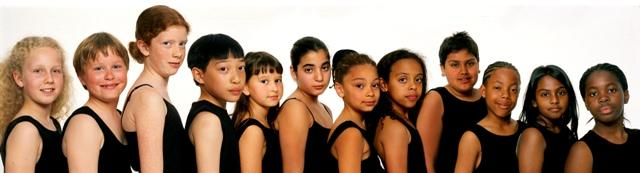
\includegraphics[width=15cm]{figures/colorskin}
\caption{Příklady druhů pigmentace kůže\cite{skincolor:obr}}
\label{colorskin}
\end{figure}

\subsection{Vnější podněty}
Problém pro identifikování chodce v~obraze může také představovat druh osvětlení scény, případně střídání dne a~noci pro venkovní kamerové systémy. Také zde hraje důležitou roli nastavení a~vlastnosti dané kamery. 

\subsection{Oblečení a~různé doplňky}
Do této kategorie spadá například zimní oblečení, které většinou zvětšuje objem či tvar těla, nebo různě rozměrné pokrývky hlavy. Chodec také může nést nějaké předměty, které mohou zakrývat jeho části těla nebo s~ním dokonce splývat. Tyto aspekty také ovlivňují správnost detekce.

\subsection{Pozice v~obraze}
Osoby se mohou nacházet libovolně v~obraze, mohou jít čelem k~ohnisku kamery nebo být zachyceny pouze z~boku. Například kamera umístěná ve výšce pouličního osvětlení v~nějakém předem určeném úhlu snímá obraz z~určité perspektivy. Tato kamera pak zajištuje velikou škálu chodců v~různém měřítku. Pro stroj tohle může být problematické. Osoby ve větším měřítku mohou být snadno detekovatelné, ovšem chodci, kteří jsou hodně vzdálení v~obraze, nikoliv. V~tomto případě také závisí na nastavení daného detektoru za cenu pomalejší a~méně přesnější detekce. 

\subsection{Pozadí (prostřední scény)}
Chodci se většinou pohybují v~komplexním venkovním prostředí. Opět, pro lidské oko může být člověk snadno identifikovatelný, a~pro doménu strojů se může tato situace jevit jako neproveditelná. Osoba v~obraze může totiž dokonale splynout s~prostředním, které se za ní nachází.  

Příklad výše zmíněných výzev a~problémů detekce najdeme na obrázku \ref{pedestrians}, který je umístěn níže. Na tomto ilustrativním obrázku najdeme osoby s~různě barevným oblečením různého tvaru. Chodci se zde nacházejí v~různém úhlu k~ohnisku kamery. 

\begin{figure}[H]
\centering
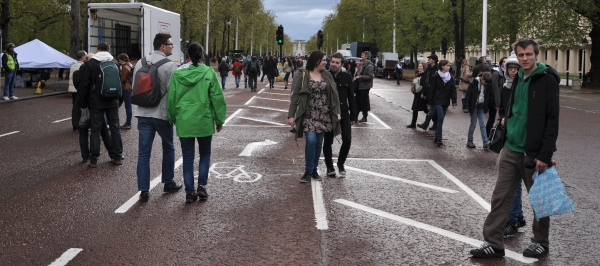
\includegraphics[width=15cm]{figures/pedestrians}
\caption{Ukázka chodců v~obraze}
\label{pedestrians}
\end{figure}